\documentclass[]{article}
\usepackage[spanish.mexico]{babel}
\usepackage[T1]{fontenc}
\usepackage[utf8]{inputenc}
%\usepackageB.\\{lmodern}
\usepackage[a4paper]{geometry}

%\usepackage{natbib}
\usepackage{cite}


%Grafico de barras
\usepackage{pgfplots}

%Graficos e imagenes
\usepackage{graphicx}


\usepackage{tikz}
\usepackage[american voltages, american currents,siunitx]{circuitikz}


\title{Introducción a la conversión de Energía}
\author{Pablo Vivar Colina}
%\date{Mayo 2018}



\begin{document}
	
%	%\usepackage[top=2cm,bottom=2cm,left=1cm,right=1cm]{geometry}


\begin{titlepage}
     \begin{center}
	
\includegraphics[width=0.09\textwidth]{UNAM}\Large Universidad Nacional Autónoma de México
        	
\includegraphics[width=0.09\textwidth]{FI}\\[1cm]
        \Large Facultad de Ingeniería\\[1cm]
       % \Large División de Ciencias Básicas\\[1cm]
         \Large Laboratorio de Fundamentos de Control(6655)\\[1cm]
         %la clave antes era:4314
         \footnotesize Profesor: Salcedo Ubilla María Leonor Ing.\\[1cm]
        \footnotesize Semestre 2019-1\\[1cm]
        
       

        \Large Práctica No. 1\\[1cm]
        
           

\Large Introdcción MATLAB
        
         %Texto a la derecha
          \begin{flushright}
\footnotesize  Grupo 2\\[0.5cm]
\footnotesize Brigada: 4\\[0.5cm]
\footnotesize Rodrigo Adrián Martínez López\\[0.5cm]
\footnotesize Vivar Colina Pablo\\[0.5cm]
 \end{flushright}
    %Texto a la izquierda
          \begin{flushleft}
        \footnotesize Ciudad Universitaria Agosto de 2018.\\
          \end{flushleft}
         
          
        %\vfill
        %\today
   \end{center}
\end{titlepage}
 %agregar portada

\maketitle

%\tableofcontents  % Write out the Table of Contents

%\listoffigures  % Write out the List of Figures

\section{Ejemplo}

Se desea conocer cual seria el incremento en grados farenheit si a una libra masa de agua se le aplica el equivalente en contenido 
energético de medio litro si un litro de helado tiene 2300kcal.

\begin{eqnarray}
  1kJ/(Kg^oC)\\
  1lb=0.4535924Kg
\end{eqnarray}

agua líquida Es $4181.3[J/gr^oK]$\\

la energía son 9627340J o es decir 9124.616672 BTU\\

Calor:\\ 

\begin{equation}
  Q=mC \Delta T
\end{equation}

Definición de BTU es igual $^oF$ a una libra\\

1BTU=1055.095282J\\

1Joule=0.0009477817BTU\\


Cada quemador de estufa convencional da 600 $[\frac{KJ}{min}]$
Combustión-> energía química a energía calorífica.\\

Primera pérdida de los procesos: perdida por diferencias caloríficos (poder calorífico superior e inferior) Ésta primer pérdida depende del tiempo de combustión, durante la combustión se genera humedad que absorbe calor y se pierde a evaporarse el agua.\\

Poder calorífico 44 $[\frac{MJ}{Kg}]$

\begin{equation}
  \frac{9.627 [MJ] [Kg]}{44[MJ]}=0.218[Kg]
\end{equation}

Esto representa el $1.09\%$ de un tanque de 20Kg de gas LP. 368 Pesos cuesta cada tanque 18.4 pesos cada Kg.\\

El $1.09\%$ del tanque cuesta 4.142 pesos.\\

\section{Ecuación de la energía Bernoulli}


\section{Ejercicio calentamiento por medio litro de helado}

Utilizando la energía que proporciona un medio litro de helado en un quemador convencional.\\

Cada quemador de estufa convencional da 600 $[\frac{KJ}{min}]$
Combustión-> energía química a energía calorífica. Se utilizarán los datos de placa de una estufa en vez de los datos proporcionados\\



\begin{equation}
   Q=mC_p\Delta T
\end{equation}

\begin{itemize}
	\item $t_1=25^oC$
	\item $C_p=4.18[\frac{KJ}{Kg^oC}]$
	\item $m=1[lb_m]*[\frac{0.454Kg_m}{1[lb_m]}]$
\end{itemize}


\begin{equation}
    p=5200[KJ/h]
\end{equation}


\begin{equation}
    \eta_{posillo} 12 \%
\end{equation}




¿Cuantos grados va a subir la temperatura y el tiempo en que se logra?


\begin{equation}
 t=(4811.6KJ)(\frac{h}{5200KJ})=0.9253076923h
\end{equation}

Teniendo en cuenta el concepto de eficiencia.\\


\begin{equation}
Q \eta_{posillo} =mC_p\Delta T 
\end{equation}

\begin{equation}
4811.6KJ*0.12=0.454KG*4.18\frac{KJ}{Kg^oC}*(t2-25^oC)
\end{equation}


\begin{equation}
\frac{4811.6KJ*0.12}{0.454KG*4.18\frac{KJ}{Kg^oC}}+25^oC=t2
\end{equation}


\begin{equation}
329.2556331^oC=t2
\end{equation}

Eficiencia normalmente con una eficiencia de una caldera industrial está alrededor de $\eta=75,78 \%$ .\\

\section{Ejemplo cocción de café}

Utilizando la energía que proporciona un medio litro de helado en un quemador convencional.\\

Se requiere que la temperatura 2 sea de $50^o$.\\

Cada quemador de estufa convencional da 600 $[\frac{KJ}{min}]$
Combustión-> energía química a energía calorífica. Se utilizarán los datos de placa de una estufa en vez de los datos proporcionados\\


\begin{equation}
Q=mC_p\Delta T
\end{equation}

\begin{itemize}
	\item $t_1=25^oC$
	\item $t_2=50^oC$
	\item $C_p=4.18[\frac{KJ}{Kg^oC}]$
	\item $m=1[lb_m]*[\frac{0.454Kg_m}{1[lb_m]}]$
\end{itemize}


\begin{equation}
p=5200[KJ/h]
\end{equation}


\begin{equation}
\eta_{posillo} 12 \%
\end{equation}




¿Cuantos grados va a subir la temperatura y el tiempo en que se logra?


\begin{equation}
t=(4811.6KJ)(\frac{h}{5200KJ})=0.9253076923h
\end{equation}

Teniendo en cuenta el concepto de eficiencia.\\


\begin{equation}
Q \eta_{posillo} =mC_p\Delta T 
\end{equation}

\begin{equation}
\frac{395.36*0.12}{0.454KG*4.18\frac{KJ}{Kg^oC}}+25^oC=t2
\end{equation}


\begin{equation}
50^oC=t2
\end{equation}

La energía utilizada fue de 395.36 $KJ$ químicos

\begin{equation}
 m_{L.P.}=(393.36KJ)(\frac{1KG_{L.P}}{44000KJ})=8.9854x10^{-3}Kg_{L.P}
\end{equation}

Costo energético del calentamiento.\\

\begin{equation}
 Costo_{energetico}=(8.9854x10^{-3}Kg_{L.P})Kg_{L.P}(\frac{19.3\$}{1 Kg_{L.P.}})=0.175\$
\end{equation}



Eficiencia normalmente con una eficiencia de una caldera industrial está alrededor de $\eta=75,78 \%$ .\\


\section{Ecuación de la continuidad}

Si un sistema o una máquina no almacena masa. La sumatoria de las mas que entran a la sumatoria de las masas que salen.\\

\begin{equation}
  \dot{\omega_1}=\dot{\omega_2}
\end{equation}


\begin{equation}
\dot{\omega_e}=\dot{\omega_s}
\end{equation}



\begin{equation}
 \omega_1=\rho_1\bar{v_1}A_1
\end{equation}

Donde $\rho$ es el peso específico.\\

\begin{equation}
\omega_1=\frac{\bar{v_1}A_1}{\sigma_1}
\end{equation}

Donde $\sigma$ es el volumen específico.\\



El agua hierve en la ciudad de México a los 93$[^oC]$

\section{Ciclo calentamiento del agua}

\begin{equation}
   _1Q_2=mc_P\Delta T
\end{equation}

\begin{equation}
_2 Q_3=mc
\end{equation}


A cada temperatura de saturación le corresponde una presión de saturación.\\

\subsection{Temperatura 20 grados}

\begin{equation}
   _1h_3=m \Delta h
\end{equation}

\begin{equation}
   h_1=h_{F1}=83.91 [\frac{KJ}{Kg}]
\end{equation}

\begin{equation}
  h_3=h_{g2}x+(1-x)h_{f2}=[(2664.39)(0.25)+(1-0.25]389.59[\frac{KJ}{Kg}]=958.59[\frac{KJ}{Kg}]
\end{equation}

Se encuentran con los valores de la tabla a 93 grados y resultando la presión de 0.07MPa

\begin{equation}
  h_{g2}=2664.39 [\frac{KJ}{Kg}]
\end{equation}

\begin{equation}
h_{f2}=389.59 [\frac{KJ}{Kg}]
\end{equation}

Calor suministrado útil.\\

\begin{equation}
_1h_3=(2Kg)(958.29-83.91)[\frac{KJ}{Kg}]=1748.76[KJ]
\end{equation}

\section{Planta de generación Eléctrica}

Una planta opera en base a un ciclo Rankine este ciclo desarrolla $90 MW_e$ brutos. Para lograr esto opera con una temperatura de sobrecalentamiento del vapor de $340[^oC]$ y una presión de 42 bar absolutos. Si la turbina de vapor tiene una eficiencia mecánica de $99.5 \%$ y una eficiencia térmica de 81 $81\%$ y el generador eléctrico enfriado por Hidrógeno tiene una eficiencia del $96\%$ además de que es enfriado por agua de mar con temperatura $16[^oC]$ la cual fija la condición de expansión final de la turbina.\\

Calcular:\\

\begin{itemize}
	\item Cual es el flujo de vapor requerido.\\
	\item La potencia del reactor si la eficiencia bruta de la central es de $31 \%$   
\end{itemize}

 \subsection{Resolución}
 
 \begin{itemize}
 	\item P= 90 $[MW_e]$
 	\item T=340 $[^oC]$
 	\item P = 42 $[bar_{abs}]$
 	\item $\eta_{mecanica}=99.5 \%$
 	\item $\eta_{termca}=81 \%$
 	\item $\eta_{electrica}=96 \%$
 	\item $T_{enfriamiento}=16^oC$
 	\item $\eta_planta=31\%$
 \end{itemize}


%\begin{figure}[h!]
	%\centering
	%\begin{circuitikz}
	%	\draw
		%(0,0) node[american nand port]{}
		%(0,-1.5) node[american nand port]{}
		%(3,0) node[american nand port]{1}
		%(3,-1.5) node[american nand port]{2}
       
  %     (0,0)--(2,0)
 %      (0,0)to[Telmech=M,n=motor](0,-3)
%	   (2,0)to[L](2,-3)
%		(0,-3)--(2,-3)
		
%		 (3,0)to[L](3,-3)
		
		
		%Segundas verticales
		%(1.6,0.3)--(1.6,-0.3)
		%(1.6,-1.2)--(1.6,-1.8)
		
		%(0,0)--(1.6,0)
		%(0,-1.5)--(1.6,-1.5)
		
		%cable a voltaje
		%(-2,-0.8)--(-1.35,-0.8)
		
		%(-2.5,-0.8) node[]{$Vin$}
		
%		;
%	\end{circuitikz}
%	\caption{}
%	\label{fig:planProb}
%\end{figure}

\begin{figure}
	\centering
	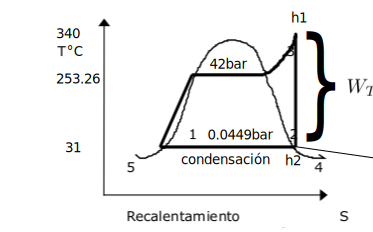
\includegraphics[width=0.85\textwidth]{SobrecalentamientoPlanta}
	\caption{Diagrama presion y Temperatura}
	\label{fig:diagPresionTemp}
\end{figure}

\begin{figure}[h!]
	\centering
	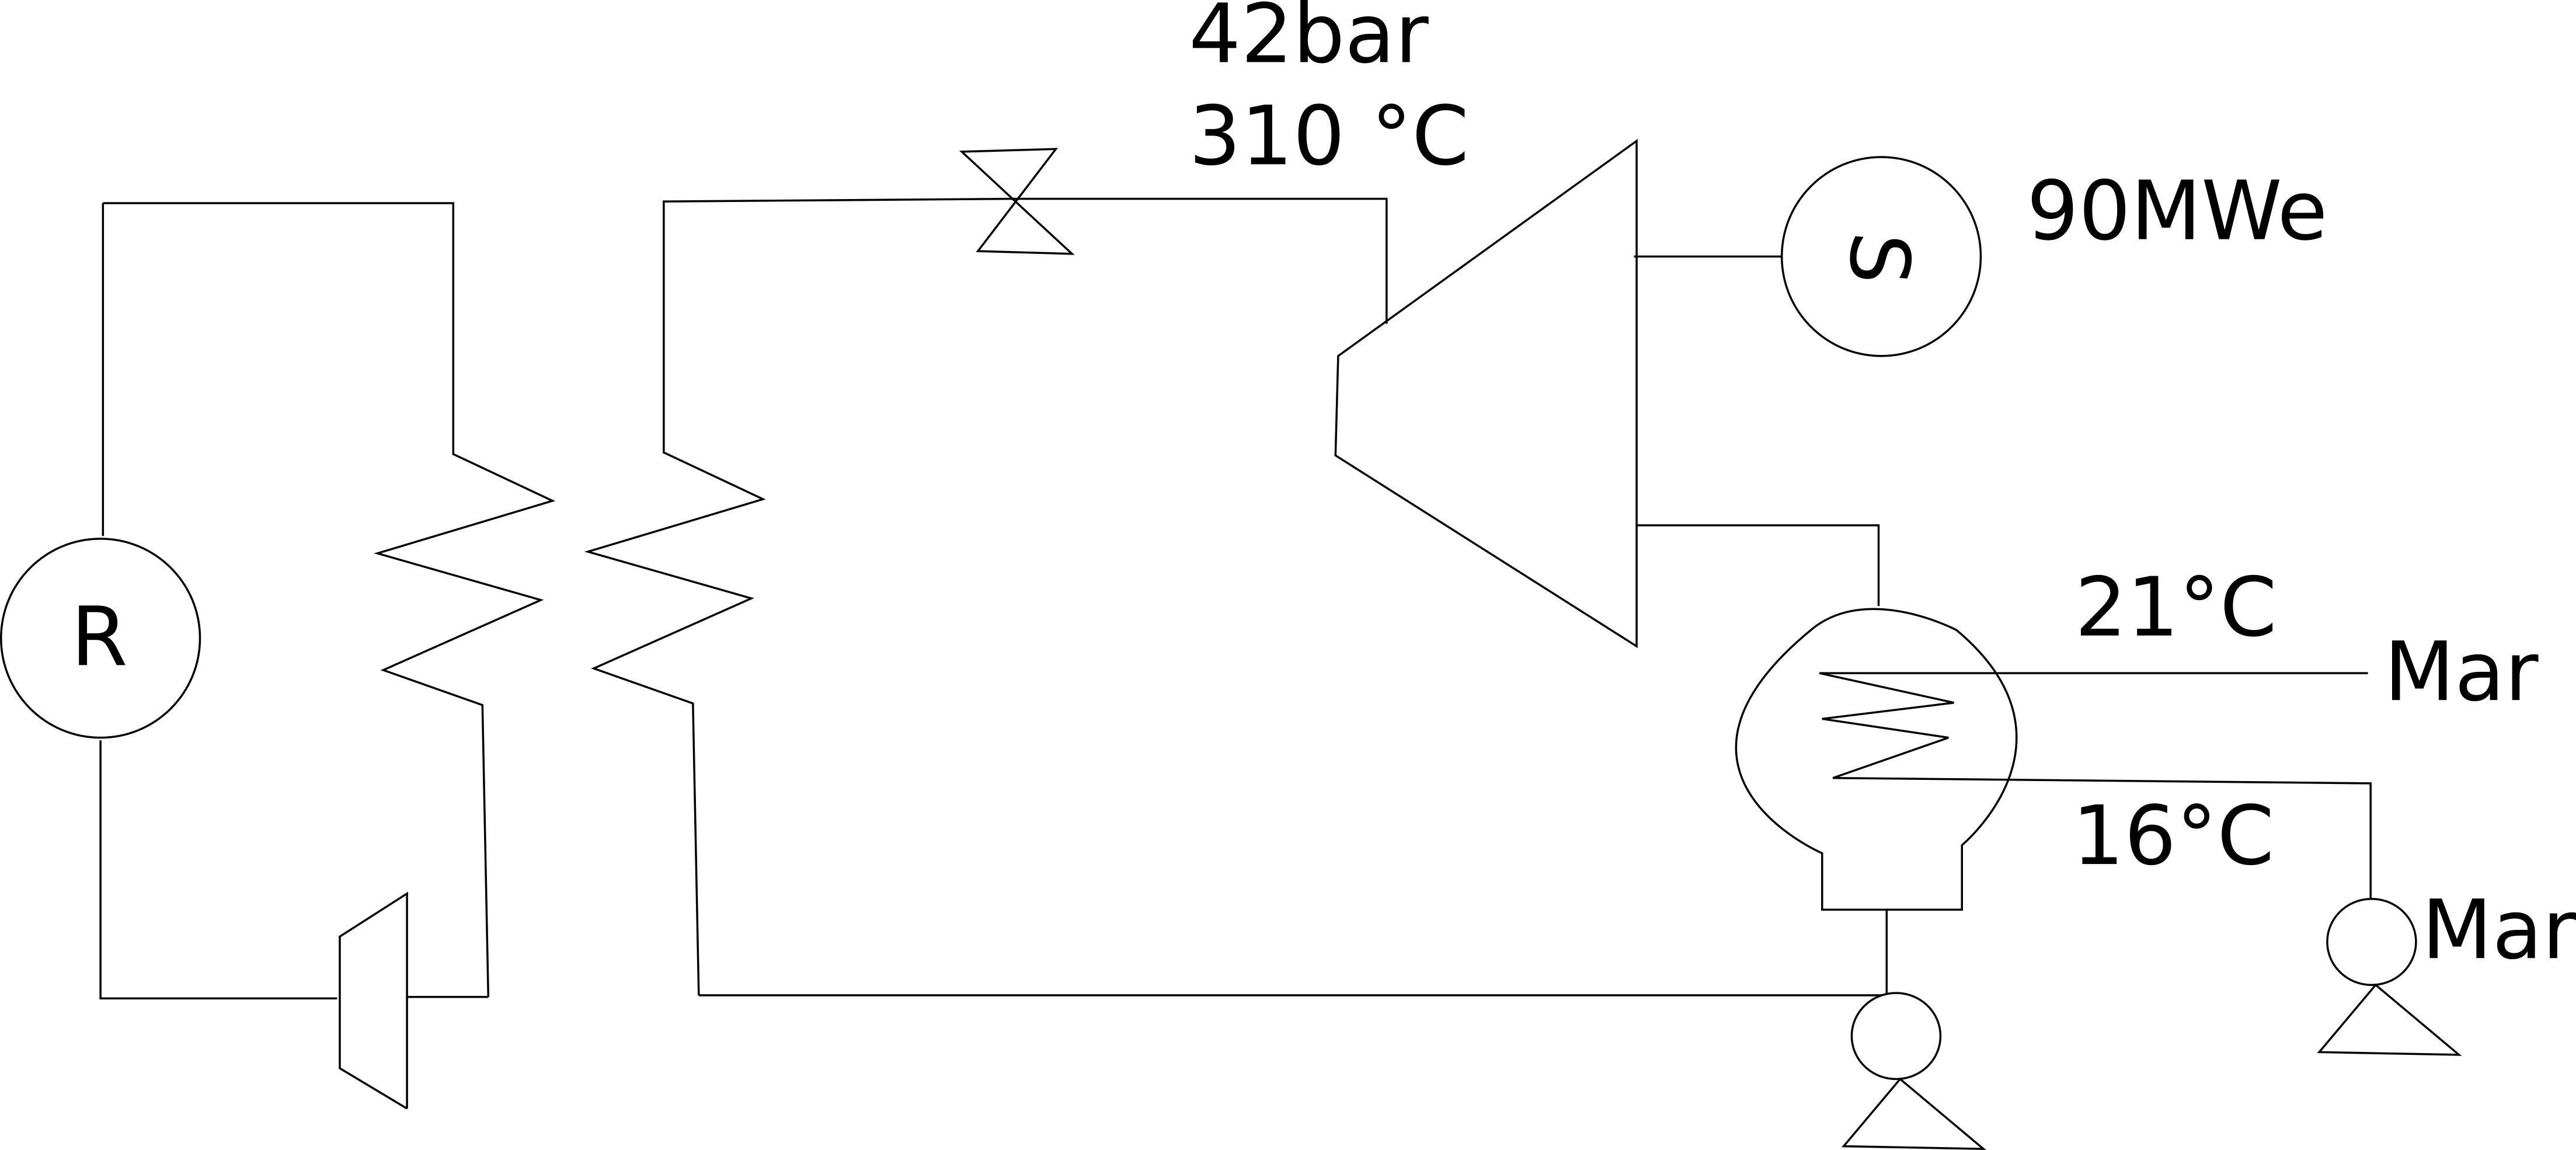
\includegraphics[width=0.85\textwidth]{diagrama.png}
	\caption{Diagrama de la Planta}
	\label{fig:diag}
\end{figure}


\begin{equation}
   W_{T.V}=\dot{m}Dh=\dot{m}(h_1-h_2)\eta_{mec}\eta_{ter}\eta_{elec}=90[MW_e]
\end{equation}

Entalpía para 340 $^oC$ y presión de 42 bar es:\\

\begin{equation}
h_1=3063.1129 [\frac{kJ}{Kg}]
\end{equation}

\begin{equation}
h_2=2314.5882 [\frac{kJ}{Kg}]
\end{equation}

\begin{equation}
\dot{m}=\frac{90[MW_e]}{(h_1-h_2)\eta_{mec}\eta_{ter}\eta_{elec}}=155.4021564[\frac{Kg}{s}]
\end{equation}

\begin{equation}
0.1554021564[\frac{Ton}{s}]=559.447763[\frac{Ton}{Hr}]
\end{equation}

\begin{equation}
   \eta_{planta}=\frac{Energia_{electrica}}{Energia_{termica}}
\end{equation}

\begin{equation}
Energia_{termica}=\frac{Energia_{electrica}}{\eta_{planta}}=290.3225806[MW_t]
\end{equation}

Para en el intercambiador de calor se busca que un líquido caliente se acerque a la temperatura de un líquido frío, se usan curvas de acercamiento paralelo o acercamiento cruzado, se considera un pinch de diferencia de 10 $^oC$.\\


\textbf{TRAER 3 EJERCICIOS DE TERMODINAMICA}

\begin{figure}[h!]
	\centering
	\includegraphics[width=0.85\textwidth]{plantaGeneradora.png}
	\caption{Diagrama de la Planta Generadora}
	\label{fig:planta}
\end{figure}

Para la figura \ref{fig:planta} vamos asignar valores correspondientes:\\

\begin{itemize}
	\item C= 14 [bar]
	\item 6v=460 mmHg
	\item Chimenea 130 $^oC$
	\item $G_1+G_2=250 [MW_e]$
	\item 5v=120 [bar] 
\end{itemize}




%\begin{thebibliography}{9}
	%\bibitem{latexcompanion} 
	%Michel Goossens, Frank Mittelbach, and Alexander Samarin. 
	%\textit{The \LaTeX\ Companion}. 
	%Addison-Wesley, Reading, Massachusetts, 1993.
	
	%\bibitem{einstein} 
	%Albert Einstein. 
	%\textit{Zur Elektrodynamik bewegter K{\"o}rper}. (German) 
	%[\textit{On the electrodynamics of moving bodies}]. 
	%Annalen der Physik, 322(10):891–921, 1905.
	
	
	%\bibitem{ebullicion} 
	 %Punto ebullición,
	%\\\texttt{http://www.cie.unam.mx/~ojs/pub/Liquid3/node8.html}
	
	
	%\bibitem{coccion} 
   %UnComo:Tiempo de cocción de los frijoles,
	%\\\texttt{https://comida.uncomo.com/articulo/tiempo-de-coccion-de-los-frijoles-34777.html}
%\end{thebibliography}






\end{document}
